\documentclass[11pt]{article}
\usepackage[margin=.78in]{geometry}
\usepackage{graphicx,amsmath,hyperref,float,microtype}
\hypersetup{colorlinks=true,allcolors=blue}
\title{Vithia 0-Vita-1: A Deterministic Context Protocol for Verifiable Scientific State Transitions}
\author{Byron P. Lee\\Biobitworks}
\date{v0.1.0 release candidate --- DOI not yet reserved}
\begin{document}
\maketitle
\begin{abstract}Scientific workflows can conflate evidence with interpretation, prediction with observation, provenance with correctness, and graph connectivity with causality. We present 0-Vita-1, a Vithia protocol separating deterministic context compilation from downstream decisions while preserving typed provenance and append-only custody. Simulated experiments test exact addressability (E0), rule inference under corruption (E1), history-sensitive context (E2), uncertainty over hidden deterministic worlds (E3), and a frozen Space Invaders snapshot set (E4A). E0, E2, and E3 are supported; E1 is partial and retains negative/null outcomes; E4A contains no decider calls. Breakpoint roots and an ordered MMR preserve identity and order, not truth. Each committed state is finite while successor context is indefinitely extensible.\end{abstract}
\section{Introduction}% CLAIM:ARCH::S0_ROLE
0-Vita-1 treats scientific type errors as a protocol problem: exact evidence identity remains separate from contextual interpretation, and Vithia-S0 context compilation remains separate from System-1 decision-making.
% CLAIM:GOV::MMR24
Hashes identify exact bytes; typed FCG edges declare relationships; breakpoint roots commit governed artifact sets; and an ordered MMR commits their sequence. These integrity mechanisms do not establish scientific truth.
\section{Formal architecture}
\[E_t\xrightarrow{S_0}C_t\xrightarrow{\Pi}P_t\xrightarrow{S_1}D_t\xrightarrow{\mathrm{world}}O_{t+1}\xrightarrow{S_0}C_{t+1}.\]
Vithia-S0 compiles source evidence into finite VitaState context. A bounded ContextPacket is projected for one downstream question; a subsequent observation creates successor evidence.
\begin{figure}[H]\centering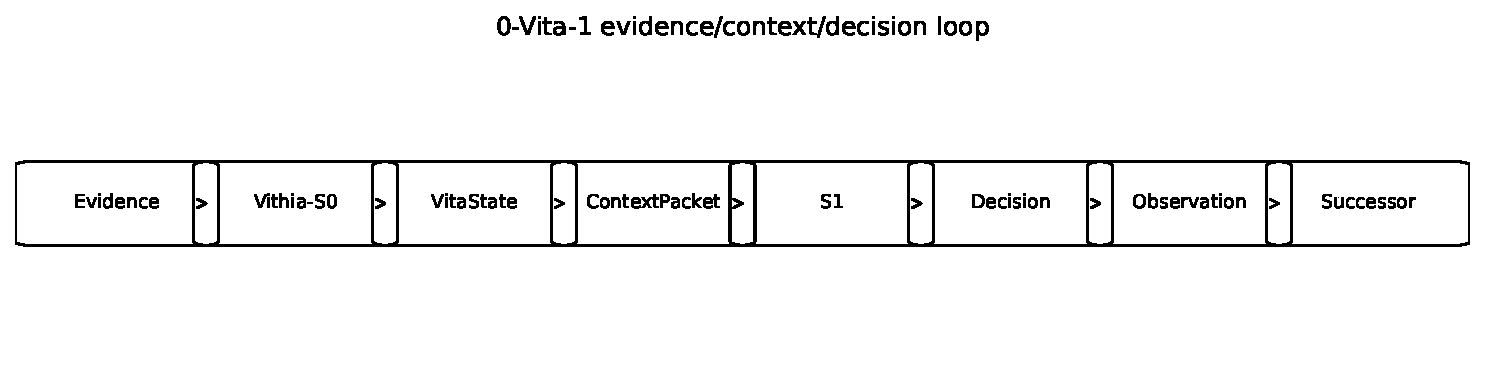
\includegraphics[width=.96\textwidth]{../figures/F1_architecture.pdf}\caption{0-Vita-1 evidence, context, decision, and successor loop}\end{figure}
\[\mathrm{identity}\neq\mathrm{meaning},\quad\mathrm{custody}\neq\mathrm{correctness},\quad\mathrm{prediction}\neq\mathrm{observation}.\]
\section{Mechanical Scientific Method}
The execution chain is question, hypothesis, preregistration, input freeze, execution, observation, analysis, claim decision, breakpoint, independent verification, and successor. Historical failures, nulls, and abstentions remain addressable.
\begin{figure}[H]\centering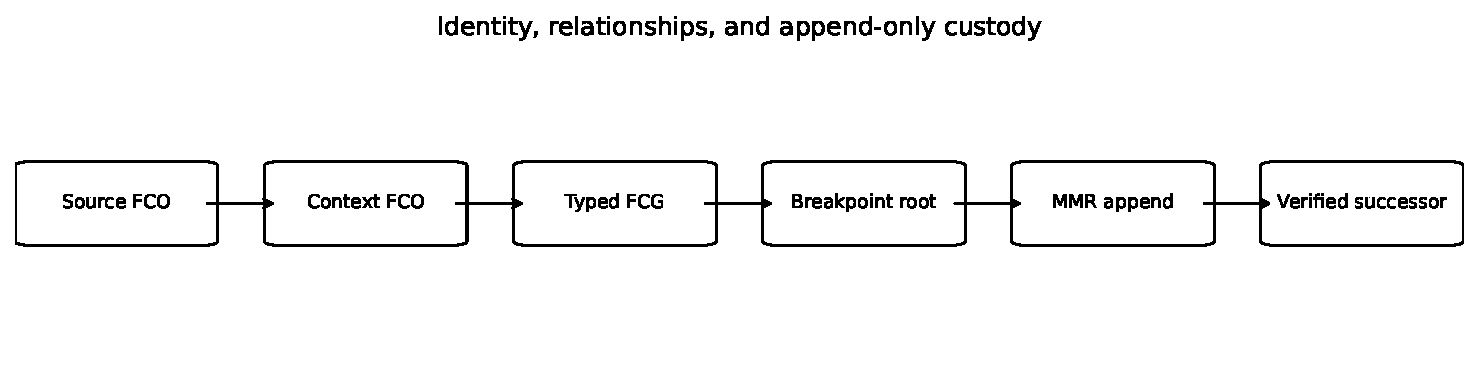
\includegraphics[width=.90\textwidth]{../figures/F2_custody.pdf}\caption{FCO, typed FCG, breakpoint, and ordered MMR custody}\end{figure}
\section{Experiment ladder}\begin{figure}[H]\centering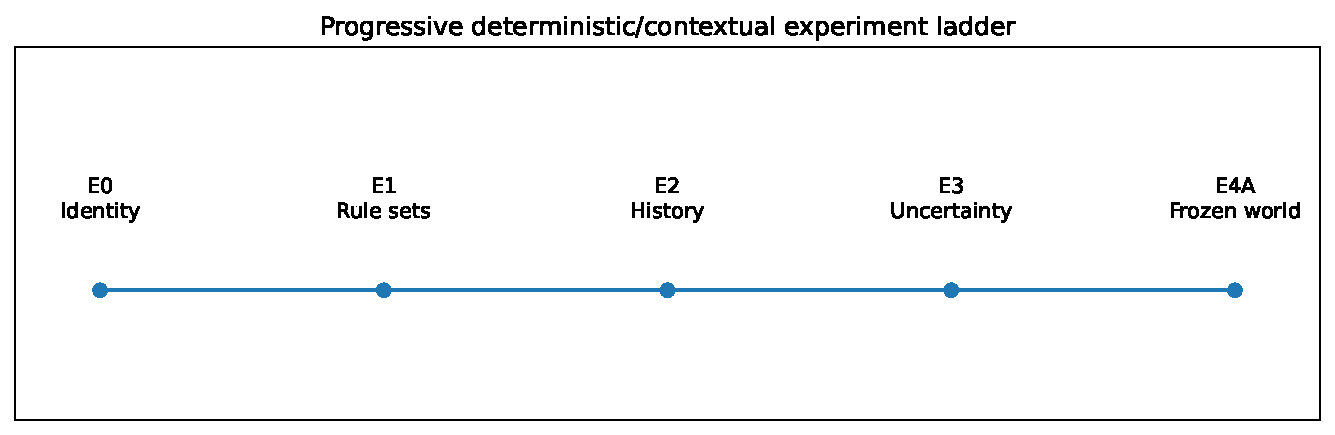
\includegraphics[width=.80\textwidth]{../figures/F3_experiment_ladder.pdf}\caption{Progressive experimental burden from identity to partial observation}\end{figure}
\section{Results}
\subsection{E0: exact addressability}% CLAIM:E0_ADDRESSABILITY::H0a
E0 is SUPPORTED. Across 10,010 rows the receipt records zero round-trip failures, zero address collisions, zero content-ID collisions, and zero address/hash-equality rows. Replay is Level 4.
\subsection{E1: rule inference}% CLAIM:E1_ECA::H1d
The independent comparison agreed on 100,352 cells with zero mismatches. E1 remains PARTIAL: H1d rank-1 fraction 0.806 is below the 0.90 threshold; Wilson 95\% CI [0.777,0.832]. H1e (p=1) and H1e-v2 (p=0.559) both FAIL\_TO\_REJECT\_H0.
\begin{figure}[H]\centering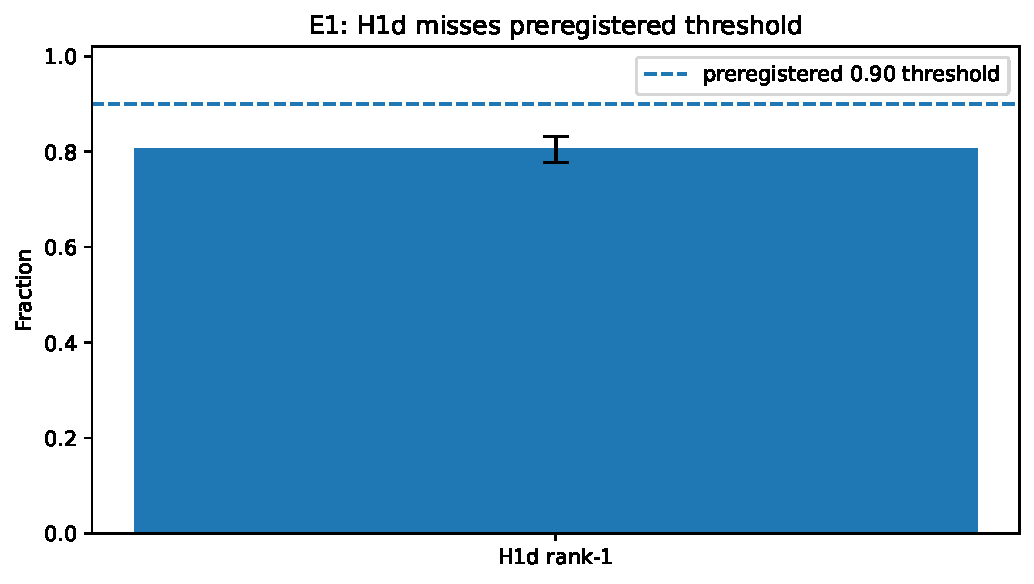
\includegraphics[width=.58\textwidth]{../figures/F4_e1_outcomes.pdf}\caption{E1 H1d and the preregistered threshold}\end{figure}
\subsection{E2: history-sensitive context}% CLAIM:E2_LIFE::H2d
E2 is SUPPORTED. Correct-history accuracy 1.000, shuffled-history 0.915, and no-history unknown rate 1.000. There are 57 same-current-atom/different-context cases. Secondary matched accuracy delta 0.087, 95\% bootstrap CI [0.019,0.163].
\begin{figure}[H]\centering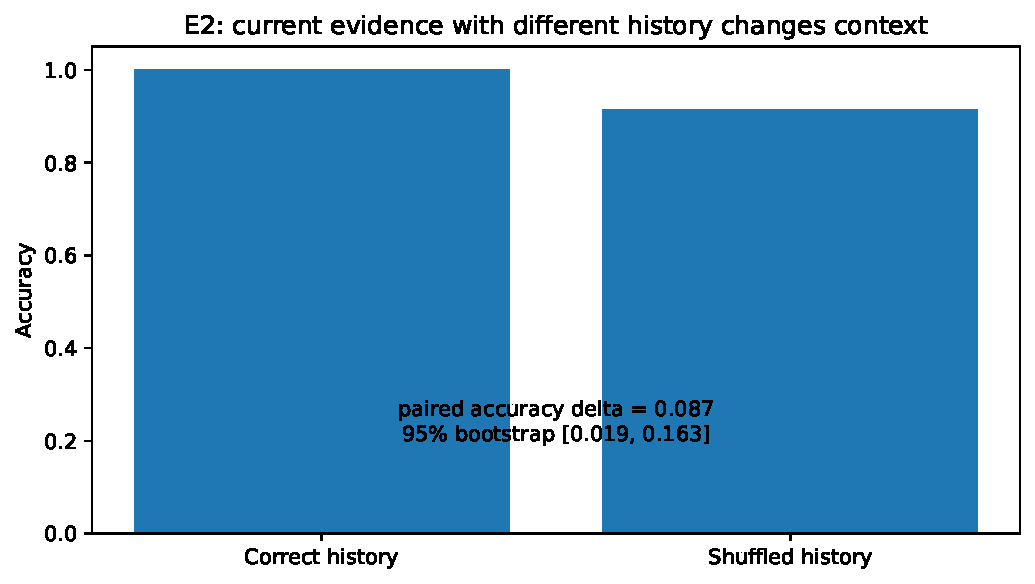
\includegraphics[width=.58\textwidth]{../figures/F5_e2_history.pdf}\caption{E2 history manipulation}\end{figure}
\subsection{E3: hidden deterministic worlds}% CLAIM:E3_MINESWEEPER::H3a
E3 is SUPPORTED with abstention. Kernel and SAT oracle agree on 28,185 eligible cells with zero disagreements; 66 states (6,484 cells) are ABSTAIN\_SIZE\_LIMIT.
% CLAIM:E3_MINESWEEPER::H3b
For 200 pairs, max-EIG realized gain is 1.9227 bits versus 1.7175 random (p=0.00605); secondary paired delta 0.205 bits, 95\% CI [0.038,0.377]. Replay remains Level 2.
\begin{figure}[H]\centering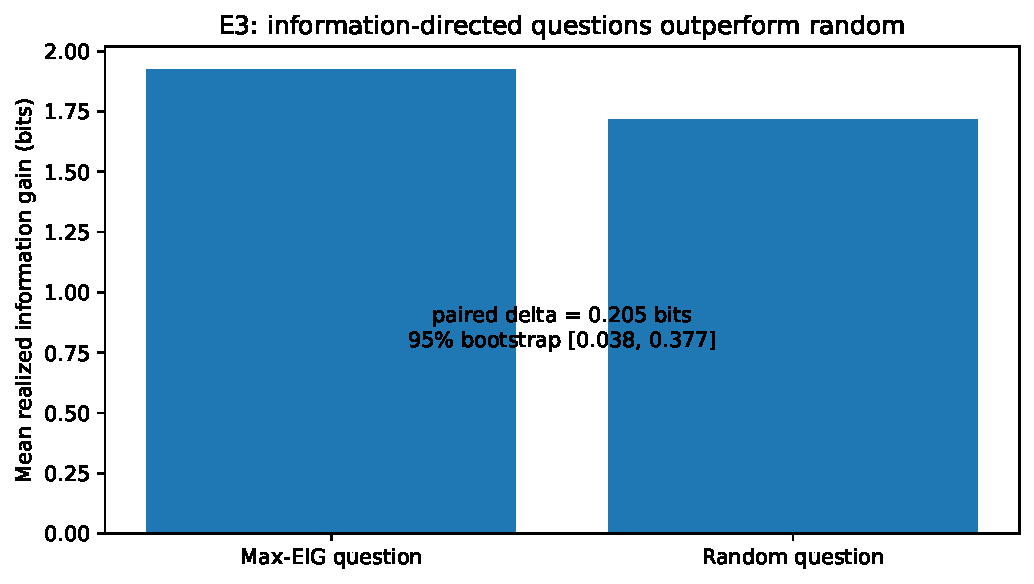
\includegraphics[width=.58\textwidth]{../figures/F6_e3_information_gain.pdf}\caption{E3 information-directed versus random questions}\end{figure}
\subsection{E4A: frozen partial observation}% CLAIM:LIMIT::E4A
E4A freezes 96 replay-verified snapshots balanced 48/48 between bomb-positive and bomb-negative strata. It is INPUT\_FROZEN\_NO\_DECIDER\_CALLS. No JEV, OpenJEV, Liquid, or Ollama/Ollarma utility claim follows.
\begin{figure}[H]\centering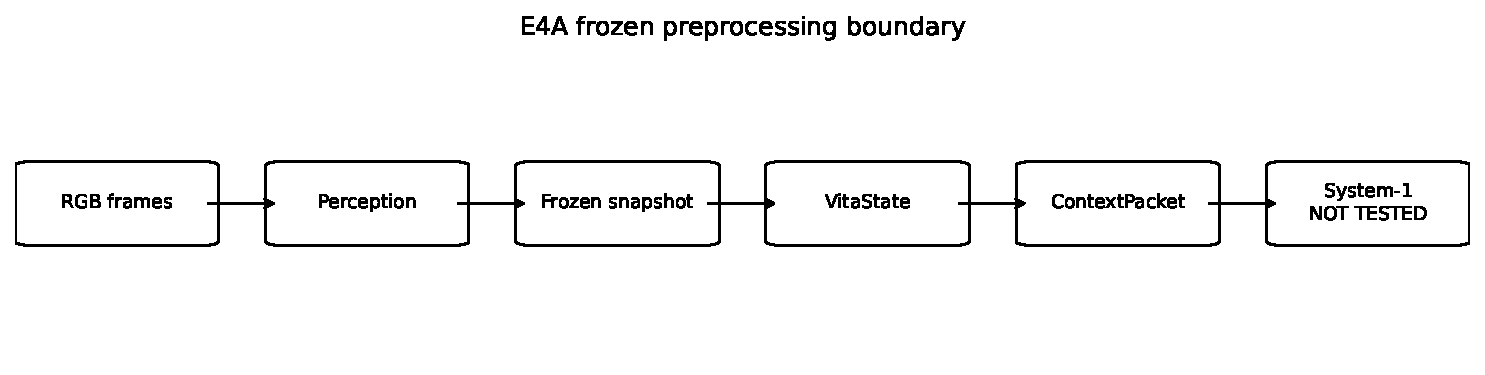
\includegraphics[width=.86\textwidth]{../figures/F7_e4a_pipeline.pdf}\caption{E4A boundary; downstream System-1 is not tested}\end{figure}
\section{Post-confirmatory statistics}% CLAIM:STAT::SECONDARY
Secondary analyses use frozen outputs and do not alter confirmatory states. E3 paired Cohen d-z is 0.168; E3 abstention fraction is 0.180.
\section{Reproducibility and custody}% CLAIM:GOV::MMR24
The publication evidence lock references UFA-JEV-BP-0024, scientific MMR size 24, root \texttt{a461def1576e4a0600cb3c738e885961678dfef300a1696e958c6b9173d76692}. Manuscript evolution uses a distinct publication MMR.
\begin{figure}[H]\centering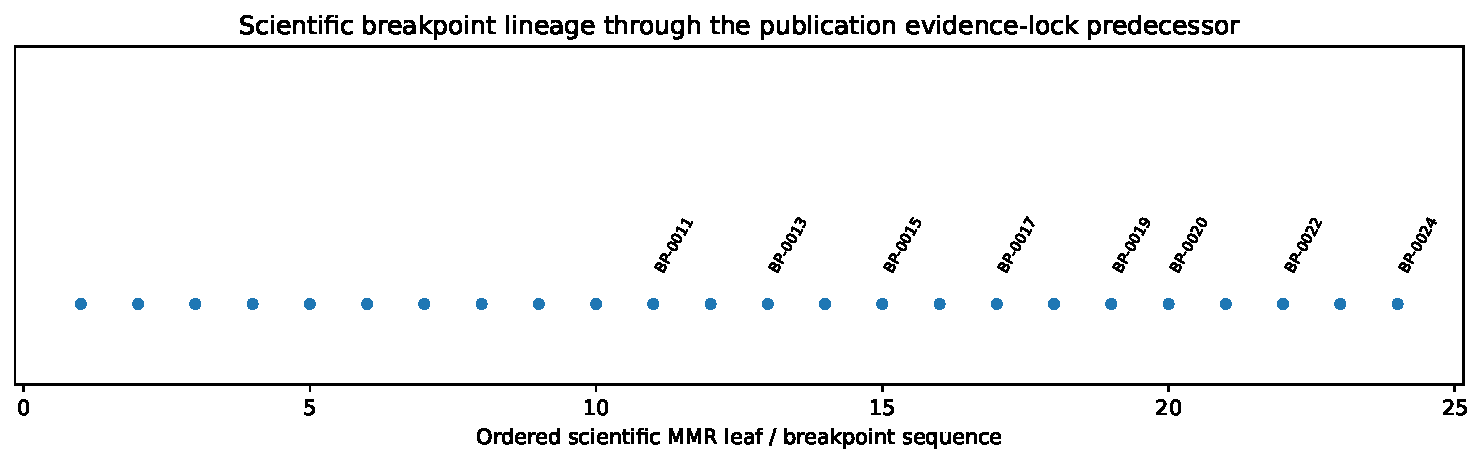
\includegraphics[width=.92\textwidth]{../figures/F8_breakpoint_timeline.pdf}\caption{Ordered scientific breakpoint lineage}\end{figure}
\section{Discussion}The results support a narrow architectural conclusion: exact evidence can remain immutable while deterministic rules produce versioned context and uncertainty remains explicit. Deterministic evidence handling does not imply a deterministic downstream model or world. Artificial Infinite Systems is structural rather than literal: every committed state is finite, while successor states can extend without rewriting predecessors.
\section{Limitations}% CLAIM:LIMIT::DELTAGSTAR
DeltaGStar is NOT\_COMPUTED; private DeltaGStar and Anticube mathematics are not disclosed and no surrogate is labeled DeltaGStar.
% CLAIM:LIMIT::CROSSHOST
Cross-host replication is DEFERRED\_NOT\_FAILED because magicPRObox was unavailable. E3 is Level-2 replay. Hosted JEV, OpenJEV, System One, Liquid, and Ollama/Ollarma utility are NOT\_TESTED. All evidence is simulated; biological transfer is NOT\_TESTED. Signatures are NOT\_SIGNED.
\section{Conclusion}0-Vita-1 provides a testable boundary between immutable evidence, deterministic context compilation, explicit uncertainty, downstream decisions, and successor observations. v0.1.0 establishes the substrate through E4A while preserving negative, null, partial, abstention, and not-tested states.
\begin{thebibliography}{3}
\bibitem{ale} Bellemare et al. The Arcade Learning Environment. JAIR 47 (2013). doi:10.1613/JAIR.3912.
\bibitem{cellpylib} Antunes. CellPyLib. JOSS 6(67) (2021). doi:10.21105/joss.03608.
\bibitem{pysat} Ignatiev et al. PySAT. SAT 2018. doi:10.1007/978-3-319-94144-8_26.
\end{thebibliography}
\end{document}
